\documentclass[twocolumn]{article}
\usepackage[english]{babel}
\usepackage[utf8]{inputenc}
\usepackage{amsmath,amssymb,physics,blindtext,graphicx}
\usepackage[a4paper,total={7.5in,10in}]{geometry}

\begin{document}
\begin{large}
\section*{Alpha decay and quantum tunnelling}
\blindtext
\begin{equation}
    \label{26mar1229}
    \frac{\hbar}{2m_\alpha}u''(r) + (V(r)-E)u(r) = 0
\end{equation}
where 
\begin{equation}
    V(r) = 
    \begin{cases}
        -V_0 + V_C(R), \quad r < R \\
        V_C(r), \qquad\qquad\,\, r\geq R
    \end{cases}
\end{equation}
and 
\begin{equation}
    V_C(r) = \frac{2(Z-2)e^2}{4\pi\epsilon_0r_j},\quad r_j\leq r < r_{j+1}
\end{equation}
where $r_j = R+j\Delta r$, $j=0,1,\dots N+1$ and $N$ is the number of barriers. The value of $V_0$ is estimated by ... in ... to be $V_0 = 134$ MeV. The radius $R$ can be calulated with the nuclear radius relationship (??):
\begin{equation}
    R = R_0\left(4^{1/3} + (A-4)^{1/3}\right)
\end{equation}
where $A$ is the mass number of the nucleus and $R_0\approx 1.2$ fm. The width of the barrier $D$ is given by $V_C(D) = E$.

\subsection*{Numerical solution}
It is convenient to write the differential equation \eqref{26mar1229} in the dimensionless form: 
\begin{equation}
    \label{26mar1412}
    \begin{split}
        &u''(\xi) + \frac{2m_\alpha D^2U}{\hbar^2}(V'(\xi)-E')u(\xi) \\ 
        &\hspace{-0.6cm}=  u''(\xi) + \alpha(V'(\xi)-E')u(\xi) = 0 
    \end{split}
\end{equation}
where $\xi=r/D$, $V'=V/U$ and $E'=E/U$. The constants $D$ and $U$ are in the units of length and energy, respectively, which makes the constant $\alpha$ dimensionless. Suitable choices $D$ and $U$ for this particular problem are $D=1$ fm and $U=1$ MeV. Since the potential is constant on the interval $(\xi_j,\xi_{j+1}) = (r_j/D,r_{j+1}/D)$, the solution on this interval is of the form:
\begin{figure}
    \centering
    \includegraphics[scale=0.5]{setup.png}
\end{figure}
\begin{equation*}
    u(\xi) = 
    \begin{cases}
        A_je^{i\omega_j\xi}+B_je^{-i\omega_j\xi},\quad E'>V'(\xi_j) \\ 
        A_je^{\omega_j\xi}+B_je^{-\omega_j\xi},\quad\,\, E'<V'(\xi_j) \\ 
    \end{cases}
\end{equation*}
where $\omega_j = \alpha\sqrt{|V'-E'|}$. When $j=N+1$, the potential has dropped below the total energy. In that region we're assuming an outgoing wave:
\begin{equation*}
    u(\xi) = Fe^{i\omega_{N+1}\xi},\quad \xi\geq \xi_{N+1}.
\end{equation*}
The unknowns $A_j$, $B_j$ and $F$, in total $2N+3$, can be found by demanding that $u$ and its derivative are continuous at the interfaces of the potential, $\xi_j$. That only gives us $2N+2$ equations but since the equation is linear, we can set $A_0 = 1$ for instance and that gives us totally $2N+3$ equations. One problem encountered when setting up the matrix for this linear system of equations was that the matrix elements, composed of exponentials of $\pm\omega_j\xi_j$, spanned several orders of magnitude because of the large value of $\omega_j\xi_j$. The best solution I found to this was to shift the system to the left so that the middle of the barrier was situated around $\xi=0$.  


\end{large}
\end{document}
